\documentclass[11pt, a4paper]{article}

% --- Packages ---
\usepackage[utf8]{inputenc}
\usepackage[T1]{fontenc}
\usepackage{geometry}
\geometry{margin=0.85in}
\usepackage{xcolor}
\usepackage{enumitem}
\usepackage{titlesec}
\usepackage{microtype}
\usepackage{tabularx}
\usepackage{booktabs}
\usepackage[most]{tcolorbox}
\usepackage{hyperref}
\usepackage{graphicx}

% --- Custom Colors ---
\definecolor{primaryBlue}{RGB}{10, 80, 160}
\definecolor{lightGray}{RGB}{245, 245, 245}

% --- Section Styling ---
\titleformat{\section}{\large\bfseries\color{primaryBlue}}{}{0em}{}[\titlerule]
\titleformat{\subsection}{\normalsize\bfseries\color{primaryBlue}}{}{0em}{}
\titlespacing*{\subsection}{0pt}{1.2ex plus 0.4ex}{0.3ex}
\setlist[itemize]{leftmargin=*, noitemsep, topsep=2pt}

% --- Custom Box for Student Info ---
\newtcolorbox{studentbox}{
    colback=lightGray,
    colframe=primaryBlue,
    boxrule=0.5pt,
    arc=4pt,
    left=15pt,
    right=15pt,
    top=10pt,
    bottom=10pt
}

% --- Markers for numbers that are not final yet ---
% \reported: from the earlier audit on the Mac, not yet reproduced on the PC
% \pending: still to be measured or checked
\newif\ifreportednoted
\newcounter{reportedfn}
\newcommand{\reported}[1]{#1\ifreportednoted\footnotemark[\number\value{reportedfn}]\else\footnote{Reported from an earlier audit on another machine; being re-checked.}\setcounter{reportedfn}{\value{footnote}}\global\reportednotedtrue\fi}
\newcommand{\resetreported}{\global\reportednotedfalse}
\newcommand{\pending}[1]{\textcolor{gray}{[pending: #1]}}
\DeclareUrlCommand\hash{\urlstyle{tt}\def\UrlBreaks{\do0\do1\do2\do3\do4\do5\do6\do7\do8\do9\do a\do b\do c\do d\do e\do f\do\_}}
\Urlmuskip=0mu plus 1mu

\begin{document}

% --- Header Section ---
\begin{center}
    {\huge \bfseries \color{primaryBlue} Dataset Datasheet} \\[0.2cm]
    {\large \textbf{Course:} DSPRO2 HS26} \\[0.1cm]
\end{center}

\vspace{0.4cm}

% --- Student & Project Information ---
\begin{studentbox}
    \begin{tabularx}{\textwidth}{l X}
        \textbf{Project Name:} & Football Analyzer \\
        \textbf{Student Names:} & Timo Tran, Johan Roth \\
        \textbf{Date:} & \today \\
        \textbf{GitHub Repository:} & \url{github.com/LittleBigFatFish/dspro2-sports-analyzer} \\
    \end{tabularx}
\end{studentbox}

\vspace{0.3cm}

\noindent We use three datasets. Each one is described with all fields of the course template. The last page compares them, gives a short zero-shot baseline and lists datasets we looked at but do not use. Run IDs refer to folders under \texttt{outputs/}; figures are made by \texttt{scripts/datasheet\_figures.py} from these folders.

% =====================================================================
\section{Dataset 1 of 3: Football Image Dataset}
\resetreported

\begin{sloppypar}\noindent\textit{Source:} audit run \texttt{20261022T191930876487Z} (recounted from \texttt{images.csv}, \texttt{boxes.csv}, \texttt{issues.csv}), overlap runs \texttt{20261103T114625435133Z} and \texttt{20261103T113605747630Z}, scoring run \texttt{20261103T122219315802Z}.\end{sloppypar}

\subsection{Dataset Overview}
\begin{itemize}
    \item \textbf{Official Name:} Football Image Dataset (GitHub \texttt{skaczylo/Football-Image-Dataset}).
    \item \textbf{Owner / Contact:} GitHub user skaczylo; no other contact given.
    \item \textbf{Short Description:} 612 frames from football matches with 10,136 boxes in YOLO format for ball, player (goalkeepers included) and referee (linesmen included). Frames come from TV broadcasts, highlight videos and one video game. Split into 512 train and 100 val images.
    \item \textbf{Version \& Date:} No release tag. Commit \hash{264212872f1bfa6a9a3413f298793474da741aec} (2026-06-23), cloned 2026-10-20 (folder date). SHA-256 of \texttt{data.yaml}: \hash{4333a70db9a10cdf147d28056bfd9674a6c1366318cb3f4c59d6baff9ebe0487}.
    \item \textbf{Reference:} \url{https://github.com/skaczylo/Football-Image-Dataset}; the README gives a BibTeX entry (skaczylo, 2026). No paper.
\end{itemize}

\subsection{Motivation and Intended Use}
\begin{itemize}
    \item \textbf{Primary Purpose:} Per the README, a ready-to-use training set for Ultralytics YOLO. Funding and other goals are not stated.
    \item \textbf{Intended Use:} Detection of ball, player and referee. We compare pretrained YOLOv8n, YOLO12n and YOLO26n at 640 and 1280 px without training; train and val share no source, so val is a fair first test. Later also fine-tuning data.
    \item \textbf{Out-of-Scope Use:} Claims about unseen matches (match count unknown); video-game frames reported as real footage; ball claims at 640 px; referee results of pretrained models (COCO has no referee class); tracking, possession, identifying people; val as a test set for any model trained on Soccana (see below).
\end{itemize}

\subsection{Composition and Coverage}
\begin{itemize}
    \item \textbf{Data Types:} Unstructured: JPEG images, one YOLO text label file per image, \texttt{data.yaml} with class names.
    \item \textbf{Population:} Professional matches 2024--25 from TV. Train: Bundesliga, Saudi league, J-League, Copa Libertadores, 2024 Community Shield. Val: Netherlands--France, Newcastle--Chelsea and Serbia U21--England U21 (highlights), and the video game eFootball PES 2021. At least 7 competitions on 3 continents. The NED--FRA overlay looks like UEFA women's branding (not checked).
    \item \textbf{Dataset Size:} 612 images, 10,136 boxes (table). Resolutions: 548 at 1920$\times$1080, 44 at 1280$\times$720, 17 at 640$\times$360, 3 at 854$\times$480. Balls per image: 118 images with none, 488 with one, 6 with two.
    \item \textbf{Known Gaps / Imbalances:} 44\% of val boxes (790 of 1,807; 43 of 100 images) are from PES 2021; real broadcast val is 57 images with 46 balls from three clips. 11.2 players per referee, 17.7 per ball. Balls are tiny: taking the shorter box side after resizing the longer image side to 640 px, 74 of 83 val balls are under 8 px (median 5.7 px); at 1280 px only 3 of 83 (median 11.4 px). With the longer box side: median 6.5 px, 66 of 83 under 8 px at 640. Missing: rain or snow, amateur and youth games, wide tactical cameras.
\end{itemize}

\begin{figure}[ht]
    \begin{minipage}[c]{0.27\textwidth}\small
        \begin{tabular}{@{}lrr@{}}
        \toprule
        & train & val \\
        \midrule
        Images & 512 & 100 \\
        Player & 7,278 & 1,566 \\
        Referee & 634 & 158 \\
        Ball & 417 & 83 \\
        Boxes & 8,329 & 1,807 \\
        \bottomrule
        \end{tabular}
    \end{minipage}\hfill
    \begin{minipage}[c]{0.72\textwidth}
        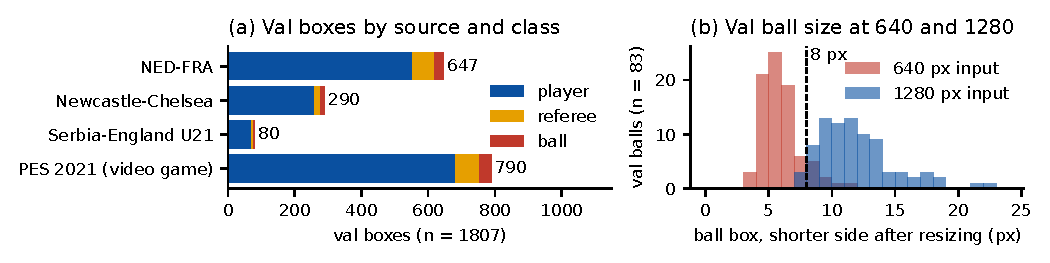
\includegraphics[width=\textwidth]{figures/football_val.pdf}
    \end{minipage}
    \caption{Football Image Dataset. Left: images and boxes per split. (a) Val boxes per source and class. (b) Val ball size after resizing to 640 and 1280 px; dashed line at 8 px.}
\end{figure}

\subsection{Sources and Collection}
\begin{itemize}
    \item \textbf{Provenance:} Public third-party footage: TV broadcasts, YouTube highlight videos (video IDs in the val file names) and one video game. The train file prefixes are export batches, not matches: \texttt{20250710\_144746} (276 images) mixes Bundesliga (SVW--BOC), Saudi league (QAD--ORO) and J-League (Nagoya); \texttt{20250710\_145737} (194) mixes Copa Libertadores and J-League (Machida--Yokohama); \texttt{20250812} (42) is the 2024 Community Shield (Man City--Man Utd). The number of matches is therefore unknown and larger than the number of batches. We found this by looking at the frames. The val images also appear in Soccana (see Initial Audit Findings), so both likely share an upstream source.
    \item \textbf{Collection Method:} Frames cut from videos. Sampling rule, frame rate, dates and tools are not documented. Val file names carry a frame index (\texttt{PES\_21\_clip\_mp4-71.jpg}).
    \item \textbf{Jurisdictions:} Broadcasts from Germany, Saudi Arabia, Japan, South America, England and two international matches. Where the data was collected and labelled is not stated.
\end{itemize}

\subsection{Labels and Targets}
\begin{itemize}
    \item \textbf{Target Definition:} Boxes with class 0 ball, 1 player (goalkeepers included), 2 referee (linesmen included). Staff and crowd are not labelled. For pretrained COCO models, player and referee count as \emph{person}, ball as \emph{sports ball}.
    \item \textbf{Labeling Process:} ``Manually annotated'' per the README; annotators, tool and guidelines unknown. Picture-in-picture insets are labelled too.
    \item \textbf{Quality Control:} None documented upstream. Ours: the audit below, a visual check of the problem cases, and a spot-check of 35 images (5 per source) by Johan \pending{error rate with n}.
\end{itemize}

\subsection{Quality Assessment (Data Audit)}
\begin{itemize}
    \item \textbf{Preprocessing Steps:} None on the raw data; \texttt{data/raw/} is never edited. Exclusion lists or corrected copies go to \texttt{data/processed/}. For inference, images are only resized (letterbox) to 640 or 1280.
    \item \textbf{Initial Audit Findings:} 0 errors, 31 warnings: 19 box edges past the image border by at most $10^{-6}$ (kept), 11 boxes with a side under 5 px (several visibly wrong) and 1 empty label. Two label errors checked by eye:
    \begin{itemize}
        \item \hash{20250710_145737_94e740}: the empty label. The README calls it an intentional background image, but it is a shot before kick-off full of players and referees.
        \item \hash{20250710_145737_9d4720}: the referee on the pitch is labelled \emph{player}; the VAR official in the inset is labelled \emph{referee}.
    \end{itemize}
    6 near-duplicate pairs within a split (dHash distance $\le 4$), none across splits. \textbf{48 of the 100 val images are also in Soccana train} (47 byte-identical, 1 near-identical), all in Soccana's \texttt{v7} group and from all four val sources (PES 20 of 43, NED--FRA 15 of 34, Newcastle--Chelsea 10 of 19, Serbia--England 3 of 4). Football train has no match. The upstream README is inaccurate: it says all images are Full HD (64 are smaller), calls the empty label intentional, and writes the folder as \texttt{football-image-dataset}, which breaks paths on case-sensitive systems.
    \item \textbf{Quality Dimensions:} \emph{Completeness:} every image has a label file; class counts match the README. \emph{Accuracy:} two known errors, 11 tiny boxes, spot-check \pending{Johan}. \emph{Consistency:} class IDs match \texttt{data.yaml}; 4 resolutions; real and video-game frames mixed. \emph{Timeliness:} matches 2024--25; commit and SHA-256 of every file recorded. \emph{What it supports:} person detection is close to solved (AP50 0.95--0.97 on real val at 1280), the ball is not: ball recall on real val is 11--30\% at 640 and 35--52\% at 1280 ($n=46$), on the video-game clip 0--22\% and 16--30\% ($n=37$).
\end{itemize}

\subsection{Legal, Ethical, and Governance}
\begin{itemize}
    \item \textbf{Sensitive Data:} Players, officials, staff and spectators are identifiable; faces are not blurred. No labels for identity, health or ethnicity. The data stays on our machines (\texttt{data/} is not committed); we publish only metrics and at most 3 frames with boxes drawn.
    \item \textbf{Compliance:} EU AI Act: our tool detects players and the ball to show match statistics. It does not identify people and is not used in a high-risk area, so we see it as minimal risk; it is coursework and not placed on the market (our assessment, to be confirmed with the supervisor). GDPR / nFADP: identifiable people are personal data. They are professionals at public events; we use the images for teaching only, store them locally and do not pass them on.
    \item \textbf{Consent \& Licensing:} \texttt{LICENSE} grants CC BY 4.0 for images and annotations. The frames come from broadcasts and a Konami video game, so the uploader cannot hold their rights; CC BY 4.0 covers the annotations at most. Consent of the people shown is not mentioned. Coursework use only, images not shared, skaczylo credited.
\end{itemize}

\subsection{Dataset Structure and Schema}
\begin{itemize}
    \item \textbf{File Formats:} JPEG images, YOLO \texttt{.txt} labels, \texttt{data.yaml}, \texttt{LICENSE}, \texttt{README.md}.
    \item \textbf{Directory Layout:} \texttt{data/raw/Football-Image-Dataset/} with \texttt{images/} and \texttt{labels/}, each split into \texttt{train/} and \texttt{val/}, kept as cloned. Audit results in \texttt{outputs/dataset\_preparation/<run id>/}.
    \item \textbf{Schema Summary:} Image and label share the base name; one line per box: \texttt{class x\_center y\_center width height}. Our \texttt{boxes.csv} has one row per box in pixels, \texttt{images.csv} one row per image with size and hashes.
    \item \textbf{Units \& Encodings:} Coordinates normalised to $[0,1]$ by image width and height. Pixel sizes are native unless 640 or 1280 is stated. Run IDs are UTC timestamps; text is UTF-8.
\end{itemize}

% =====================================================================
\section{Dataset 2 of 3: Soccana V1}
\resetreported

\begin{sloppypar}\noindent\textit{Source:} the Hugging Face card at the pinned revision, \texttt{data/raw/}\allowbreak\texttt{soccana\_v1.source.json}, audit run \texttt{20261103T113452946760Z}, overlap run \texttt{20261103T114625435133Z}, scoring run \texttt{20261103T122219315802Z}.\end{sloppypar}

\subsection{Dataset Overview}
\begin{itemize}
    \item \textbf{Official Name:} Soccana\_player\_ball\_detection\_v1 (card title ``Soccana\_prb\_v1''), file \texttt{V1.zip}.
    \item \textbf{Owner / Contact:} Hugging Face user Adit-jain; processing code in the GitHub repository \texttt{Adit-jain/Soccer\_Analysis}.
    \item \textbf{Short Description:} Detection data for player, referee and ball, merged from Roboflow Universe datasets and, per the card, SoccerNet frames, video-game renders and public footage. Most images were cut into tiles of 160 to 640 px (SAHI slicing) and capped per source. YOLO and COCO labels; train and test split.
    \item \textbf{Version \& Date:} Revision \hash{9e768912f134a7d68b58ddc9db9bcd3f6fbe39b7} (created 2025-07-26, last change 2025-08-28). \texttt{V1.zip}: 1,341,080,234 bytes, SHA-256 \hash{58f28e4c75b440f2ce67a239b9e44121976f55ae612a9eb8c07dcefb107dc1b6}, downloaded 2026-11-03 and matched against the published digest.
    \item \textbf{Reference:} No paper. Card: \url{https://huggingface.co/datasets/Adit-jain/Soccana_player_ball_detection_v1}; code: \url{https://github.com/Adit-jain/Soccer_Analysis}.
\end{itemize}

\subsection{Motivation and Intended Use}
\begin{itemize}
    \item \textbf{Primary Purpose:} Per the card, a starting point for a general football object detector; a subset of a collection of over one million images.
    \item \textbf{Intended Use:} Training data only, without the \texttt{v7} group and the excluded images; we train with and without it. Zero-shot check on 500 seeded full frames from train.
    \item \textbf{Out-of-Scope Use:} Results on its test split (it overlaps with train); results on tiles or renders presented as broadcast performance; claims about generalisation; sharing the data.
\end{itemize}

\subsection{Composition and Coverage}
\begin{itemize}
    \item \textbf{Data Types:} Unstructured: images with YOLO text labels, plus COCO JSON files.
    \item \textbf{Population:} Football scenes from seven source groups, named in the file names (table). 8,250 images (71\%) are tiles (\texttt{\_sahi\_<N>\_} in the name, size at most $N\times N$); 3,423 are full frames, most resized to 640$\times$640, 15 at 7680$\times$4320. The card also names an eighth Roboflow set and SoccerNet, but no file name points to them. Share of video-game renders \pending{not marked in the files}.
    \item \textbf{Dataset Size:} 11,673 images (8,677 train, 2,996 test), not the 25,000 on the card; the Hugging Face viewer lists 23,372 rows. 64,648 boxes: 55,704 player, 5,344 referee, 3,600 ball.
    \item \textbf{Known Gaps / Imbalances:} 3,501 empty label files (background tiles). The mix follows fixed caps per source, not content. Tiles change object sizes: in full frames the ball's shorter side at 640 px has a median of 8.1 px (1,267 of 2,710 under 8 px), larger than in the other two datasets. Match dates and leagues unknown.
\end{itemize}

\begin{center}\small
\begin{tabular}{@{}llrrrr@{}}
\toprule
Group & Roboflow source (card) & Images & Tiles & Test & Ball \\
\midrule
\texttt{v7} & Football Player Detection KUCAB & 3,546 & 2,900 & 1,046 & 635 \\
\texttt{v3} & Detect Players DGXZ0 & 3,475 & 2,800 & 975 & 945 \\
\texttt{v12} & Player Detection GKLRL & 1,725 & 1,500 & 425 & 323 \\
\texttt{v2\_temp} & VA Project & 1,290 & 950 & 290 & 503 \\
\texttt{tbd\_v2} & Football Detection Test & 797 & 0 & 20 & 653 \\
\texttt{v5\_temp} & Football EITPT & 700 & 0 & 200 & 491 \\
\texttt{spt\_v2} & Soccer Player Tracker & 140 & 100 & 40 & 50 \\
\bottomrule
\end{tabular}
\end{center}

\subsection{Sources and Collection}
\begin{itemize}
    \item \textbf{Provenance:} Third-party public sources, mainly Roboflow Universe uploads (each with its own licence, origin often unclear). The \texttt{v7} group contains 48 of the 100 Football val images, including PES frames, so it shares an upstream source with the Football dataset. Against SoccerNet test: no exact match and no SoccerNet file name.
    \item \textbf{Collection Method:} Per the card: COCO source sets $\rightarrow$ SAHI slicing at 160/320/640/1280 px with 20\% overlap $\rightarrow$ image limit per source $\rightarrow$ class name mapping $\rightarrow$ COCO to YOLO. Augmented images (background only, noise, rotation) were added.
    \item \textbf{Jurisdictions:} Not stated.
\end{itemize}

\subsection{Labels and Targets}
\begin{itemize}
    \item \textbf{Target Definition:} Player (goalkeepers included), referee, ball. \texttt{data.yaml}: 0 Player, 1 Ball, 2 Referee. The card's class table (2 = ball) is wrong; its mapping section matches the files. We remap to the Football IDs in our processed copies.
    \item \textbf{Labeling Process:} Taken over from the source datasets, which used different names and rules (e.g.\ ``Team-A'', ``Joueur'', ``Gardien''), and merged by name. Slicing cuts boxes at tile borders.
    \item \textbf{Quality Control:} Upstream mentions only a visualisation script. Our 20 overlays per class: players 20 of 20 correct; balls mostly correct, 2 unclear; referees mostly correct, with one likely goalkeeper and one rotated augmented tile.
\end{itemize}

\subsection{Quality Assessment (Data Audit)}
\begin{itemize}
    \item \textbf{Preprocessing Steps:} None on the raw data (two Ultralytics label caches were not extracted). Exclusion lists and the class remap go to \texttt{data/processed/}.
    \item \textbf{Initial Audit Findings:} 81 box rows outside the image in 75 images (the COCO file keeps them: 64,729 rows). \textbf{The test split leaks:} 135 test images have a twin in train (16 byte-identical, 28 mirrored, 91 near-identical at dHash distance $\le 4$; 24 checked by eye, all real), and test is augmented. The audit excludes 209 images. The overlap check excludes 71 images: 48 Football val copies and 24 tiles that near-match the foggy SoccerNet clip SNMOT-132 (6 checked, all false positives; one image in both). Whole-image hashing cannot find crops, and \texttt{v7} has 2,900 tiles, so we drop the whole \texttt{v7} group.
    \item \textbf{Quality Dimensions:} \emph{Completeness:} three image counts (card, viewer, files). \emph{Accuracy:} overlays mostly correct (above). \emph{Consistency:} conflicting class tables; mixed tile sizes; \texttt{data.yaml} points to the uploader's own disk. \emph{Timeliness:} match dates unknown; revision and zip hash pinned. \emph{What it supports:} training only; zero-shot ball recall on full frames is 14--18\% at 640 and 15--19\% at 1280 ($n=395$), person AP50 0.46--0.58, much lower than on the other two datasets.
\end{itemize}

\subsection{Legal, Ethical, and Governance}
\begin{itemize}
    \item \textbf{Sensitive Data:} As for the Football dataset; close-up tiles show faces larger. No identity labels. Data stays local; at most 3 frames with boxes published.
    \item \textbf{Compliance:} As for the Football dataset (EU AI Act minimal risk, to be confirmed; GDPR / nFADP: professionals at public events, teaching use only, stored locally, not passed on).
    \item \textbf{Consent \& Licensing:} No licence on the Hugging Face page or card, so all rights are reserved by default. The source datasets have their own Roboflow licences \pending{per-source check}. Consent of the people shown is not mentioned. Used only for training in this course, not shared; author and sources credited.
\end{itemize}

\subsection{Dataset Structure and Schema}
\begin{itemize}
    \item \textbf{File Formats:} One ZIP with JPEG images, YOLO \texttt{.txt} labels, COCO JSON files and \texttt{data.yaml}.
    \item \textbf{Directory Layout:} \texttt{data/raw/soccana\_v1/} (the ZIP's \texttt{V1/} folder) with \texttt{images/} and \texttt{labels/}, each split into \texttt{train/} and \texttt{test/}, plus \texttt{coco\_train\_annotations/}, \texttt{coco\_test\_annotations/} and \texttt{samples/}. Download record in \texttt{data/raw/soccana\_v1.source.json}.
    \item \textbf{Schema Summary:} YOLO: one label file per image, one line per box. COCO: \texttt{images}, \texttt{annotations} and \texttt{categories} linked by IDs. The source group is the file name prefix.
    \item \textbf{Units \& Encodings:} YOLO coordinates normalised to $[0,1]$; COCO boxes in pixels as $[x, y, w, h]$. Class IDs differ from the Football dataset (ball 1 instead of 0).
\end{itemize}

% =====================================================================
\section{Dataset 3 of 3: SoccerNet Tracking 2023}
\resetreported

\begin{sloppypar}\noindent\textit{Source:} Cioppa et al.\ (2022); \texttt{data/raw/}\allowbreak\texttt{sn\_tracking\_2023.source.json}; view runs \texttt{20261103T113130922060Z} (1 fps) and \texttt{20261103T113141540915Z} (1 per 5\,s) in \texttt{outputs/}\allowbreak\texttt{soccernet\_view/}; their audits \texttt{20261103T113334952545Z} and \texttt{20261103T113351992092Z}; scoring run \texttt{20261103T122219315802Z}.\end{sloppypar}

\subsection{Dataset Overview}
\begin{itemize}
    \item \textbf{Official Name:} SoccerNet-Tracking, 2023 challenge release (\texttt{SoccerNet/SN-Tracking-2023}).
    \item \textbf{Owner / Contact:} The SoccerNet team (A.~Cioppa, S.~Giancola et al.; University of Liège, KAUST); \url{https://www.soccer-net.org}.
    \item \textbf{Short Description:} 30-second clips from broadcasts of professional football games with tracking labels: a box and a track ID per object and frame. Each track has a role (player, goalkeeper, referee, ball, other) and often a jersey number. Each clip has JPEG frames, a MOT ground-truth file, \texttt{gameinfo.ini} and \texttt{seqinfo.ini}.
    \item \textbf{Version \& Date:} Revision \hash{3777f456d908570e10b19e7354744640e77c351e} (uploaded 2026-09-06). \texttt{test.zip}: 8,711,601,474 bytes, SHA-256 \hash{46b248735ac068abc8c0d53c7a868826fa73a9b3b633295c6957f04bb7576716}, downloaded 2026-11-03 and matched against the published digest. \texttt{train.zip} (9,575,523,385 bytes) and \texttt{challenge2023.zip} (5,311,510,942 bytes) not downloaded yet.
    \item \textbf{Reference:} A.~Cioppa et al., ``SoccerNet-Tracking: Multiple Object Tracking Dataset and Benchmark in Soccer Videos'', CVPR Workshops 2022, arXiv:2204.06918; \url{https://huggingface.co/datasets/SoccerNet/SN-Tracking-2023}.
\end{itemize}

\subsection{Motivation and Intended Use}
\begin{itemize}
    \item \textbf{Primary Purpose:} A research benchmark for multi-object tracking in football broadcasts, used in the yearly SoccerNet challenges.
    \item \textbf{Intended Use:} Our main detection test set at 1 frame per second (1,470 frames from 49 clips; 294 frames at 1 per 5\,s for CPU runs), later for tracking (milestone M3). The train split is for fine-tuning later.
    \item \textbf{Out-of-Scope Use:} Claims beyond the three test games; treating consecutive frames as independent samples; identifying players (jersey numbers are labelled); views other than the main broadcast camera.
\end{itemize}

\subsection{Composition and Coverage}
\begin{itemize}
    \item \textbf{Data Types:} Unstructured JPEG frames with semi-structured text (MOT \texttt{.txt}, \texttt{.ini}).
    \item \textbf{Population:} Broadcast games of professional football. Test: 3 games (IDs 7, 8 and 11 with 16, 19 and 14 clips). Each clip is linked to an annotated action (e.g.\ corner) and its game time.
    \item \textbf{Dataset Size:} Test: 49 clips of 750 frames, 36,750 frames at 1920$\times$1080 and 25\,fps, 564,547 boxes, 34,129 of them ball. Tracks: 975 player, 63 goalkeeper, 102 referee, 65 ball, 6 other. 1 fps view: 1,470 frames with 19,417 player, 1,799 referee and 1,368 ball boxes, plus 52 ignored boxes. Train: \reported{57 clips}, not downloaded.
    \item \textbf{Known Gaps / Imbalances:} Only 3 test games, so uncertainty is estimated per clip, not per frame; frames in a clip are nearly identical. At 1 fps, 114 frames have no ball and 12 have two real balls. The ball's shorter side at 640 px has a median of 5.0 px (1,280 of 1,368 under 8 px). League, season and weather coverage \pending{not in the clip files}.
\end{itemize}

\subsection{Sources and Collection}
\begin{itemize}
    \item \textbf{Provenance:} Broadcast videos of professional games collected and labelled by the SoccerNet team (see paper). No exact copy and no SoccerNet file name in Soccana.
    \item \textbf{Collection Method:} Clips of 30\,s at 25\,fps, 1920$\times$1080, from the main broadcast camera.
    \item \textbf{Jurisdictions:} Not stated on the Hugging Face page or in the clip files \pending{leagues}.
\end{itemize}

\subsection{Labels and Targets}
\begin{itemize}
    \item \textbf{Target Definition:} Boxes with track IDs; each track's role is in \texttt{gameinfo.ini}. Our mapping: player and goalkeeper $\rightarrow$ player, referee $\rightarrow$ referee, ball $\rightarrow$ ball. \emph{other} (6 tracks of medical staff in clips SNMOT-133 and SNMOT-188) is ignored: predictions on it count neither as correct nor as false.
    \item \textbf{Labeling Process:} Done by the dataset authors; details in the paper. All confidence values are 1.
    \item \textbf{Quality Control:} Described in the paper. Our 20 overlays per class: class labels correct; a few people are not labelled.
\end{itemize}

\subsection{Quality Assessment (Data Audit)}
\begin{itemize}
    \item \textbf{Preprocessing Steps:} None on the raw data. Our converter (\texttt{sports\_analyzer/soccernet.py}) writes YOLO views to \texttt{data/processed/soccernet/} (\texttt{test\_1fps}, \texttt{test\_per5s}): roles mapped, \emph{other} on an ignore list, frames hard-linked. Only the test split is local, so the train/test game split is recorded, not checked (train games \reported{4, 6 and 9}).
    \item \textbf{Initial Audit Findings:} 1 fps view: 0 errors; 101 warnings for boxes at the image edge (rounding, harmless) and 11 boxes under 5 px. The role spelling is inconsistent (``goalkeepers team left'' vs ``goalkeeper team right''). MOT coordinates count from 0.
    \item \textbf{Quality Dimensions:} \emph{Completeness:} all 49 clips have 750 frames and labels. \emph{Accuracy:} labels correct in the overlays, a few people missing. \emph{Consistency:} one resolution and frame rate. \emph{Timeliness:} 2023 challenge release; revision and zip hash pinned. \emph{What it supports:} person AP50 0.86 at 1280 for all three models (clip bootstrap, e.g.\ YOLO12n 0.84--0.88); ball recall 8--16\% at 640 and 29--32\% at 1280 ($n=1{,}368$).
\end{itemize}

\subsection{Legal, Ethical, and Governance}
\begin{itemize}
    \item \textbf{Sensitive Data:} Broadcast footage with identifiable players, officials, medical staff and spectators; faces not blurred. Jersey numbers per track together with the game make players identifiable; we do not use them. Data stays local; at most 3 frames with boxes published.
    \item \textbf{Compliance:} As for the Football dataset (EU AI Act minimal risk, to be confirmed; GDPR / nFADP: professionals at public events, teaching use only, stored locally, not passed on).
    \item \textbf{Consent \& Licensing:} The Hugging Face repository has no licence file or card and is not gated, so we treat it as all rights reserved. The videos belong to the broadcasters. SoccerNet terms of use \pending{Johan}. We cite the paper, use the data for coursework only and do not share it.
\end{itemize}

\subsection{Dataset Structure and Schema}
\begin{itemize}
    \item \textbf{File Formats:} ZIP with JPEG frames, MOT text files and \texttt{.ini} files.
    \item \textbf{Directory Layout:} \texttt{data/raw/sn\_tracking\_2023/test/SNMOT-<id>/}: frames in \texttt{img1/}, labels in \texttt{gt/gt.txt}, detections in \texttt{det/}, plus \texttt{gameinfo.ini} (game, action, track roles) and \texttt{seqinfo.ini} (size, frame rate, length).
    \item \textbf{Schema Summary:} \texttt{gt.txt}: one row per box: frame, track ID, left, top, width, height, confidence and three unused columns. \texttt{gameinfo.ini} links track IDs to roles.
    \item \textbf{Units \& Encodings:} Boxes in pixels, counted from 0; frames numbered from 1 at 25\,fps. Our YOLO views use normalised coordinates and the Football class IDs.
\end{itemize}

% =====================================================================
\section{Comparison of the Three Datasets}
\resetreported

\noindent Sources as given in each part. Ball size: median shorter side of the ball box after resizing the longer image side to 640 px.

\begin{center}\small
\begin{tabularx}{\textwidth}{>{\raggedright\arraybackslash}p{2.1cm} >{\raggedright\arraybackslash}X >{\raggedright\arraybackslash}X >{\raggedright\arraybackslash}X}
\toprule
 & \textbf{Football Image Dataset} & \textbf{Soccana V1} & \textbf{SoccerNet Tracking 2023 (test)} \\
\midrule
Images & 612 & 11,673 (card: 25,000) & 36,750 frames, 49 clips; 1,470 at 1 fps \\
Boxes & 10,136 & 64,648 & 564,547; 22,584 at 1 fps \\
Ball boxes & 500 & 3,600 & 34,129; 1,368 at 1 fps \\
Ball size at 640 & 5.6 px (456 of 500 under 8 px) & 8.1 px in full frames & 5.0 px at 1 fps \\
Classes & ball 0, player 1, referee 2 & player 0, ball 1, referee 2 & roles: player, goalkeeper, referee, ball, other \\
Resolution & 640$\times$360 to 1920$\times$1080 & tiles 160 to 640 px; full frames up to 7680$\times$4320 & 1920$\times$1080 \\
Image type & full frames; broadcast and video game & 71\% tiles; broadcast, renders & consecutive broadcast frames \\
Split structure & train 512 / val 100, no shared source & train 8,677 / test 2,996; 135 test images leak & test 49 clips from 3 games; train not local \\
Overlap & 48 val images in Soccana \texttt{v7} & 71 excluded, \texttt{v7} dropped & none exact with Soccana \\
Licence & CC BY 4.0 (annotations at most; frames third-party) & none stated (all rights reserved) & no licence text; cite paper \\
Our role & pretrained comparison; fine-tuning & training only & main test set; tracking (M3) \\
\bottomrule
\end{tabularx}
\end{center}

\begin{figure}[ht]
    \centering
    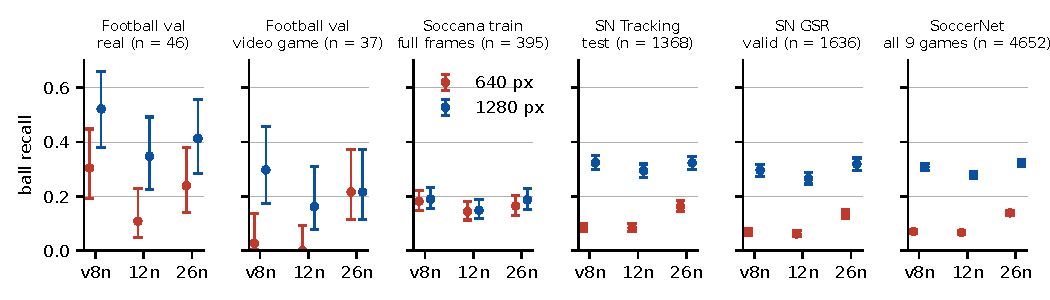
\includegraphics[width=\textwidth]{figures/ball_recall.pdf}
    \caption{Zero-shot ball recall (confidence 0.25, IoU 0.5, Wilson 95\% intervals) of pretrained YOLOv8n, YOLO12n and YOLO26n (Ultralytics assets v8.4.0, SHA-256 in \texttt{models/MANIFEST.json}) at 640 and 1280 px. Scoring run \texttt{20261103T122219315802Z}. Football val is split into real and video game.}
\end{figure}

\noindent The same run also scores YOLO26n at 1920 px and with its NMS-free head. A higher input size (1920) raises ball recall on real footage (Football real .46, SoccerNet .35) but not on the video-game clip or Soccana. The NMS-free head gives slightly lower recall, except on real Football at 640 (.30 vs .24).

\noindent CPU latency on the 100 Football val images (median ms at 640 / 1280; run \texttt{20261103T121139897997Z}): YOLOv8n 33.7 / 86.4, YOLO12n 44.0 / 156.1, YOLO26n 38.7 / 92.7, YOLO26n NMS-free 36.1 / 90.6.

\subsection{Considered, Not Used}
\begin{center}\small
\begin{tabularx}{\textwidth}{>{\raggedright\arraybackslash}p{4.2cm} >{\raggedright\arraybackslash}p{3.0cm} >{\raggedright\arraybackslash}X}
\toprule
\textbf{Dataset} & \textbf{Licence / access} & \textbf{Why not now} \\
\midrule
SoccerNet Game State Reconstruction 2025 (Somers et al., CVPRW 2024) & GPL-3.0, not gated, about 35\,GB & Pitch positions, roles, teams and jersey numbers; too large for now. Planned for milestone M4. \\
MCG-NJU SportsAction / MultiSports (Li et al., ICCV 2021) & CC BY-NC 4.0, gated & Only players performing an action are boxed and the ball is not labelled. \\
SkillCorner opendata & MIT, credit requested & Tracking data and events of 10 A-League matches (2024/25), no images. Later for the analysis metric. \\
\bottomrule
\end{tabularx}
\end{center}

\subsection{Credits}
\begin{itemize}
    \item Football Image Dataset by skaczylo, \url{https://github.com/skaczylo/Football-Image-Dataset} (CC BY 4.0).
    \item Soccana V1 by Adit-jain, \url{https://huggingface.co/datasets/Adit-jain/Soccana_player_ball_detection_v1}, and the Roboflow Universe datasets listed on its card.
    \item SoccerNet-Tracking: A.~Cioppa, S.~Giancola, A.~Deliège, L.~Kang, X.~Zhou, Z.~Cheng, B.~Ghanem, M.~Van Droogenbroeck, CVPR Workshops 2022, arXiv:2204.06918.
    \item SoccerNet Game State Reconstruction: V.~Somers et al., CVPR Workshops 2024, arXiv:2404.11335. MultiSports: Y.~Li et al., ICCV 2021, arXiv:2105.07404. SkillCorner opendata: \url{https://github.com/SkillCorner/opendata}.
    \item YOLOv8, YOLO12 and YOLO26 weights and the \texttt{ultralytics} package by Ultralytics, AGPL-3.0, \url{https://github.com/ultralytics/ultralytics}.
\end{itemize}

\end{document}
